% !TeX encoding = UTF-8
% !TeX program = pdflatex
% !TeX spellcheck = it_IT

\documentclass[Lau,binding=0.6cm]{sapthesis}

\usepackage{microtype}
\usepackage{float}
\usepackage[italian]{babel}
\usepackage[utf8]{inputenx}

\usepackage{listings} %Per inserire codice


\usepackage{hyperref}
\hypersetup{pdftitle={Sapthesis class example},pdfauthor={Francesco Biccari}}

% Remove in a normal thesis
\usepackage{lipsum}
\usepackage{curve2e}
\definecolor{gray}{gray}{0.4}
\newcommand{\bs}{\textbackslash}

% Commands for the titlepage
\title{Rappresentazione JavaScript di entità OWL e loro proprietà in linguaggio Graphol}
\author{Valerio Longo}
\IDnumber{1655653}
\course{Ingegneria dei Sistemi Informatici}
\courseorganizer{Facoltà di ingegneria dell'informazione, informatica e statistica}
\courseorganizer{Dipartimento di Ingegneria informatica, automatica e gestionale “Antonio Ruberti”}
\AcademicYear{2017/2018}
\copyyear{2018}
\advisor{Prof. Maurizio Lenzerini}
\authoremail{longo.1655653@studenti.uniroma1.it}

\versiondate{\today}



\begin{document}

\frontmatter

\maketitle


\tableofcontents

\frontmatter
\chapter{Introduzione} L'obiettivo di questo progetto è quello di dare all'utente la possibilità di scegliere una tra le varie entità di un'ontologia e vederla disegnata a schermo con tutti i suoi ruoli, attributi, superclassi, sottoclassi e loro relative funzionalità, tutto in stile Graphol. Per prima cosa viene fatto partire un programma Java che esamina un file Owl attraverso le OWLAPI e ne genera uno nuovo di estensione json. Dopodiché, su browser, un file HTML tramite JavaScript e Jquery genera un'interfaccia di upload per il file  json e la selezione delle entità presenti al suo interno. Il layout è generato attraverso Cytoscape.js, una libreria JavaScript per la visualizzazione di grafi.\\ Questa relazione è divisa in tre parti. La prima discute in maniera introduttiva OWL, Graphol e gli strumenti utilizzati, la seconda è incentrata sulla parte Java del progetto e l'ultima invece analizza dettagliatamente il codice HTML e Javascript.
\\Prima di iniziare però c'è da chiarire che molti dei tools utilizzati per questo progetto non erano mai stati studiati durante il percorso di studi, pertanto se ci fossero imprecisioni nelle modalità di realizzazione o in qualche parte del codice queste sarebbero nient'altro che ingenuità dettate dalla poca esperienza.
\mainmatter


\chapter{Parte 1 - Linguaggi e strumenti utilizzati}
\section{OWL}
OWL (da Web Ontology Language) è una famiglia di linguaggi utilizzati per rappresentare esplicitamente il significato e la semantica di termini e relazioni tra gli stessi. Esistono quindi varie versioni del linguaggio, che differiscono molto tra di loro. In questo progetto sono stati utilizzati file con sintassi funzionale OWL 2. L'utilizzo di OWL ha per obiettivo quello di rappresentare, ragionare, dedurre e collegare informazioni appartenenti allo stesso contesto. Segue quindi che analizzare informazioni provenienti da contesti differenti porterebbe a conclusioni totalmente errate ed è quindi necessario delimitare chiaramente il loro dominio di interesse. La rappresentazione di tale dominio è detta \textbf{ontologia}. Al suo interno vi gravitano \textbf{entità, espressioni e assiomi}.
\\Le \textbf{entità} sono gli elementi atomici di un ontologia. Sono identificati da un IRI e possono essere classi, individui e proprietà. 
	Una classe è per esempio p:Uomo, la quale può essere usata per rappresentare l'insieme di tutti gli uomini a livello 			estensionale.	
    Un individuo invece è p:Lucio, usato per rappresentare a livello intensionale un uomo chiamato "Lucio". 
	Una proprietà (o relazione) può essere p:padreDi, usata per rappresentare il ruolo di padre.
\\Le \textbf{espressioni} invece rappresentano complesse nozioni interne al dominio di interesse. Per esempio, un'espressione descrive un insieme di uomini accomunati dalla caratteristica di essere padri.
\\Infine, gli \textbf{assiomi} sono affermazioni prese indiscutibilmente come vere ed utilizzate come premesse per ragionamenti più complessi. Un esempio di assioma può essere: la classe p:Uomo è una sottoclasse della classe p:Persona.
\\Queste tre categorie sintattiche sono usate per esprimere la parte logica delle ontologie OWL. Queste sono interpretate attraverso una precisa semantica che permette di estrarre deduzioni molto utili. Per esempio, se un individuo p:Lucio è istanza 
della classe p:Uomo, e p:Uomo è sottoclasse di p:Persona, allora da ciò si può dedurre che p:Lucio è istanza anche di p:Persona.
È quindi facilmente intuibile che serva una metodologia per estrarre informazioni da un'ontologia e con Java, tramite le OWL API questo compito riesce piuttosto bene.

\section{OWLAPI}
OWL API è un API Java open source per la manipolazione e l'analisi di ontologie OWL. Esso è compatibile con moltissimi ragionatori, fondamentali per questo progetto in quanto servono per \textbf{dedurre} assiomi. In questo progetto è stato utilizzato HermiT come ragionatore nella sua versione 1.3.8.500. OWL API è fortemente legato da dipendenze, perciò è stato praticamente d'obbligo l'utilizzo di Maven come software di gestione per la parte Java del progetto. 

\section{Graphol}
Graphol è un linguaggio visuale per le ontologie. Un'ontologia viene considerata come un grafo con \textbf{nodi} (ruoli, concetti, attributi) e \textbf{archi} (collegamenti). Questi vengono disegnati con uno stile molto semplice e intuitivo che permette di evitare l'analisi di complesse strutture sintattiche.

\begin{figure}[H]
\centering
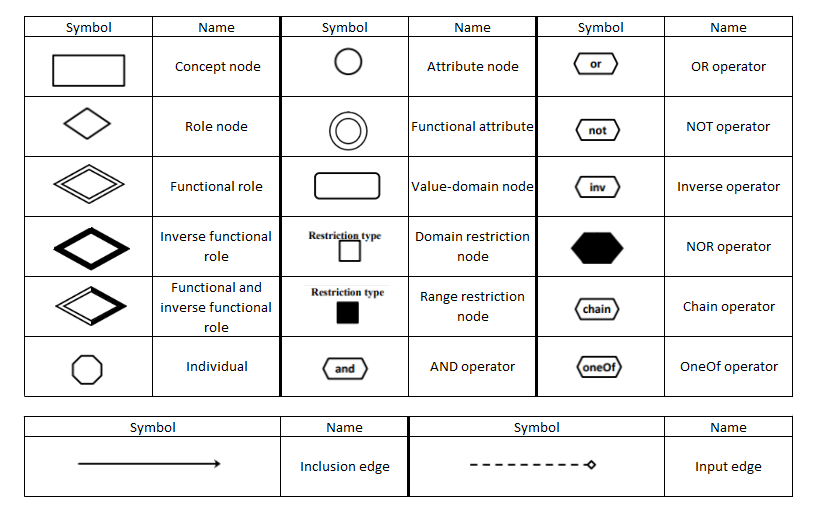
\includegraphics[width=1\textwidth]{final}\\[3ex]
\caption{Alcuni simboli di Graphol, ispirati a quelli dei diagrammi ER}
\label{fig:largenenough}
\end{figure}
I versi degli archi possono avere diverse configurazioni a seconda del tipo di partecipazione di ogni nodo.
Una partecipazione obbligatoria (Mandatory partecipation) impone che ogni oggetto nelle istanze di un concetto (atomico o complesso) è anche nelle istanze del dominio ( oppure del range) di un ruolo. Una partecipazione di tipizzazione (che può essere di dominio o di range) specifica il "tipo" degli oggetti che vengono istanziati nel dominio (o nel range) di un ruolo.
\begin{figure}[H]
\centering
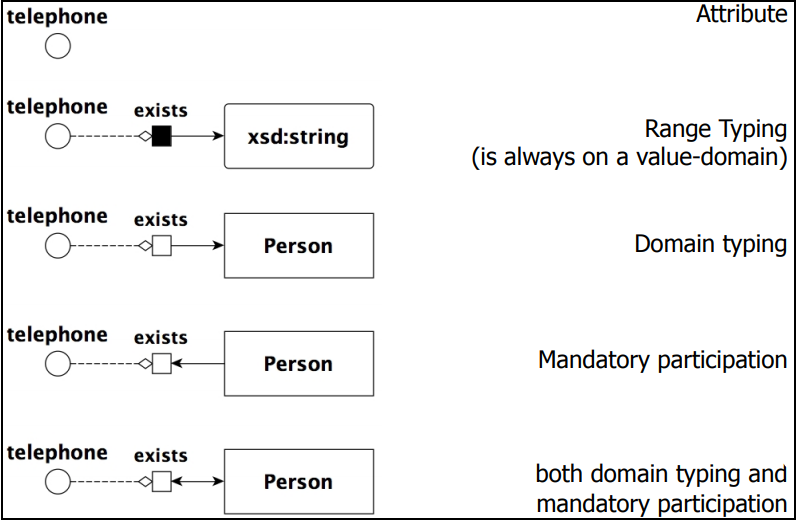
\includegraphics[width=1\textwidth]{mandeopt}\\[3ex]
\caption{diverse configurazioni di partecipazione tra un concetto ed un attributo, il discorso è simile anche tra concetti e ruoli}
\label{fig:largenenough}
\end{figure}
Ora che sono state chiarite le basi e gli intenti di questo progetto, andiamo ad analizzarlo più approfonditamente. Per evitare di rendere questa relazione troppo prolissa, verrà riportato il codice solo per le varie inizializzazioni, mentre per quanto riguarda i singoli algoritmi di estrapolazione, analisi e visualizzazione verranno solamente descritti e saranno riportati solo i procedimenti più interessanti.

\chapter{Parte 2 - Da .owl a .json }
L'IDE sul quale è stata sviluppata la parte Java del progetto è NetBeans. Come già accennato, le OWL API sono tanto utili quanto legate a dipendenze, a causa di ciò è stato necessario l'utilizzo di Maven. Inoltre è stata di aiuto \textit{simple-JSON}, una libreria per la creazione e gestione del formato JSON. L'input di questo programma è un file owl scelto dall'utente e l'output è un file JSON che ha la seguente struttura:
\begin{verbatim}
{   
    "Concepts":[
        {"CONCETTO1":{"Super_Concepts":["SUPERCONCETTI"]}},
        {"CONCETTO2":{
            "Mandatory_Attributes":["ATTRIBUTI_MANDATORI"],
            "Sub_Concepts":[["GRUPPO_DI_SOTTOCONCETTI1"],["GRUPPO_DI_SOTTOCONCETTI2"]],
            "Optional_Roles":["RUOLI_OPZIONALI"]}
        },
        {"CONCETTO3":{"Mandatory_Roles":["RUOLI_MANDATORI"]}}
    ],
    "Roles":[
        {"RUOLO1":{
        	"Domain":["CONCETTO_DOMINIO"],
        	"Range":["CONCETTO_RANGE"],
        	"ObjectProperty":["Functional"]
        	}
        }
    ],
    "Attributes":[
        {"ATTRIBUTO1":{
        	"Domain":["CONCETTODOMINIO"],
        	"ObjectProperty":"Functional",
        	"Mandatory_in":["CONCETTO"]
        	}
        }
    ]
}
\end{verbatim}
La classe GenerateJson.java è la sola e unica di questa parte del progetto. È composta dal main e da tre metodi  \textit{LavoraConcetti, LavoraRuoli, LavoraAttributi}. Come si può intuire dal nome, ognuno di questi tre metodi "lavora" sul singolo gruppo di entità dell'ontologia, estraendo informazioni dall'input.

\section{Main}
Prima di tutto bisogna inizializzare il programma e fornirgli il file owl.
\begin{verbatim}
JFileChooser chooser = new JFileChooser();
FileNameExtensionFilter filter = new FileNameExtensionFilter("OWL FILES", "owl");
chooser.setFileFilter(filter);
chooser.setMultiSelectionEnabled(false);
chooser.setFileSelectionMode(JFileChooser.FILES_AND_DIRECTORIES);
int retval = chooser.showOpenDialog(new JFrame("GenerateJson"));
\end{verbatim}
Utilizzando il componente JFileChooser viene creato un JFrame che permette all'utente di scegliere l'input. Viene permesso di selezionare solamente file con estensione owl. Il ritorno di \textit{chooser.showOpenDialog()} viene catturato.\\
\begin{verbatim}
File file;
if (retval == JFileChooser.APPROVE_OPTION) {
   try { 
       file = chooser.getSelectedFile();
       OWLOntologyManager manager = OWLManager.createOWLOntologyManager();
       OWLOntology o = manager.loadOntologyFromOntologyDocument(file);


       JSONObject obj = new JSONObject();

       //INIZIO ELABORAZIONE DATI PER I CONCETTI
       JSONArray arrayconcetti = new JSONArray();
       LavoraConcetti(arrayconcetti,o);
       obj.put("Concepts", arrayconcetti);
       //FINE ELABORAZIONE DATI PER I CONCETTI

       //INIZIO ELABORAZIONE DATI PER I RUOLI
       JSONArray arrayruoli = new JSONArray();
       LavoraRuoli(arrayruoli,o);
       obj.put("Roles", arrayruoli);
       //FINE ELABORAZIONE DATI PER I RUOLI

       //INIZIO ELABORAZIONE DATI PER GLI ATTRIBUTI
       JSONArray arrayattributi = new JSONArray();
       LavoraAttributi(arrayattributi,o);
       obj.put("Attributes", arrayattributi);
       //FINE ELABORAZIONE DATI PER GLI ATTRIBUTI


       //SCRITTURA DEL RISULTATO SU  FILE SU DEKSTOP.
       FileWriter localfile = new FileWriter("/Users/theta/Desktop/prova.json") 
       localfile.write(obj.toJSONString());
       System.out.println("Successfully Copied JSON Object to File...");
       System.out.println("\nJSON Object: " + obj);
                
     }
   catch (Exception ex) {
       JOptionPane.showMessageDialog(
       		new JFrame("Exception"), "Error opening file!", "Error!", retval
       		);
       System.exit(1);
   }
}
if(retval == JFileChooser.CANCEL_OPTION){
     JOptionPane.showMessageDialog(
     		new JFrame("operazione annullata"), "operazione annullata", "Error!", retval
     		);
     System.exit(1);
}
\end{verbatim}
In sostanza, nel caso di esito positivo nella scelta del file di input, viene creato \textit{JSONObject obj} e \textit{OWLOntology o}. Quest'ultimo non è altro che il file owl convertito in ontologia grazie alle OWLAPI ed è l'elemento sul quale faremo le operazioni di analisi, infatti è argomento di tutti e tre i metodi statici. L'oggetto \textit{obj} invece, non è altro che il contenuto del file (all'inizio vuoto) di output. Esso verrà riempito in tre step, grazie ai tre metodi statici. Per ogni gruppo di entità (concetti, ruoli e attributi) viene creato un array che verrà poi aggiunto ad \textit{obj} al termine della chiamata di ogni metodo. Infine \textit{obj} viene scritto su un nuovo file .json.
\\Nel caso ci fosse un problema nell'accettazione dell'input oppure un annullamento durante la scelta del file, il programma termina.

\section{Il metodo LavoraConcetti}
\begin{verbatim}
private static void LavoraConcetti(JSONArray arrayconcetti,OWLOntology o) 
\end{verbatim}
Questo metodo statico ha come obiettivo quello di riempire \textit{arrayconcetti} con tutti i concetti presenti in \textit{o} ed i loro relativi collegamenti.
Per fare ciò è necessario un ragionatore:
\begin{verbatim}
		OWLReasonerFactory rf = new org.semanticweb.HermiT.ReasonerFactory();
		OWLReasoner r = rf.createReasoner(o);
		// RIEMPIO LISTA CON STRINGHE DI TUTTI I CONCETTI       
		List<String> listanomiConcetti = new LinkedList<String>();
		List<OWLClass> listanomiOWLConcetti = new LinkedList<OWLClass>();
		
		
		for (OWLClass cls : o.getClassesInSignature()){
	     	listanomiConcetti.add(cls.getIRI().getFragment());
    	 	listanomiOWLConcetti.add(cls);                       
		}
\end{verbatim}
Viene creato il ragionatore, vengono create le liste con all'interno tutti i concetti. Adesso si opera su ogni elemento di una delle due liste.
\begin{verbatim}
for (int i = 0; i < listanomiConcetti.size(); i++) {
      JSONObject oggettoConcetto = new JSONObject();
      JSONObject infoOggettoConcetto = new JSONObject();
      String nomeConcetto = listanomiConcetti.get(i);
      //GESTIONE ATTRIBUTI
      List<String> MandAttrlist= new LinkedList<String>(); 
      //...ALGORITMO DI ESTRAPOLAZIONE DEGLI ATTRIBUTI ATTRAVERSO IL RAGIONATORE
      if(!MandAttrlist.isEmpty()){
      	infoOggettoConcetto.put("Mandatory_Attributes", MandAttrlist);
      	}
      
      //GESTIONE RUOLI MANDATORI
      List<String> MandRolelist = new LinkedList<String>();
      //...ALGORITMO DI ESTRAPOLAZIONE DEGLI RUOLI MANDATORI..
      if(!MandRolelist.isEmpty()){
      	infoOggettoConcetto.put("Mandatory_Roles", MandRolelist);
      	}
      //continua....	
      
}
\end{verbatim}

In sostanza, per ogni concetto vengono create delle liste per ogni tipo di dato (superclassi, sottoclassi, attributi, ruoli mandatori, ruoli opzionali ecc..). Successivamente, attraverso il ragionatore, si estraggono le informazioni per ogni tipo di dato e vengono inserire all'interno della relativa lista. Se la lista ha almeno un elemento, deve essere inserita in  \textit{infoOggettoConcetto} insieme alla descrizione del tipo di dato.

\begin{verbatim}
oggettoConcetto.put(nomeConcetto, infoOggettoConcetto);
arrayconcetti.add(oggettoConcetto);
\end{verbatim}

Così facendo viene fatto side-effect e viene riempito l'array che è stato dato come input nel main.
\\Appena terminata l'esecuzione del metodo, arrayconcetti viene inserito in obj.
\section{Il metodo LavoraRuoli}
\begin{verbatim}
private static void LavoraRuoli(JSONArray arrayruoli,OWLOntology o)
\end{verbatim}
Ciò che viene fatto qui è molto simile a quello svolto da \textit{LavoraConcetti()}, cambia solamente il contenuto delle liste per rispettare la formattazione del file json vista ad inizio capitolo.
\\\begin{verbatim}
List<String> listanomiRuoli = new LinkedList<String>();
List<OWLObjectProperty> listaowlruoli = new LinkedList<OWLObjectProperty>();
for (OWLObjectProperty cls : o.getObjectPropertiesInSignature()){
      listaowlruoli.add(cls);
      listanomiRuoli.add(cls.getIRI().getFragment());
}
\end{verbatim}
Ciò che effettivamente cambia è il soggetto. Infatti qui vengono analizzati tutti gli elementi dell'ontologia con proprietà \textit{getObjectPropertiesInSignature()}.
\\La struttura è sempre la stessa, per ogni ruolo corrente, viene creata una serie di liste, ognuna con al suo interno le informazioni utili alla sua rappresentazione Graphol. Una volta raggruppate le informazioni in liste, vengono inserite nell'\textit{JSONObject infoOggettoRuolo}. Successivamente
\begin{verbatim}
oggettoRuolo.put(nomeRuolo, infoOggettoRuolo);
arrayruoli.add(oggettoRuolo);
\end{verbatim}
A fine chiamata, arrayruoli (contente tutti i ruoli dell'ontologia) viene inserito in obj.

\section{Il metodo LavoraAttributi}
\begin{verbatim}
private static void LavoraAttributi(JSONArray arrayattributi, OWLOntology o) 
\end{verbatim}
\begin{verbatim}
for (OWLDataProperty cls : o.getDataPropertiesInSignature()){
    listaowlattributi.add(cls);
    listanomiAttributi.add(cls.getIRI().getFragment());
}
\end{verbatim}

Questa volta, la lista di attributi viene fornita tramite \textit{o.getDataPropertiesInSignature()}, ed i suoi elementi verranno analizzati prima per vedere se sono funzionali(se sì, in che modo), poi per vedere quali sono i domini, i range e per ultimo se sono mandatori. Poi, una volta inserite tutte le liste in \textit{infoOggettoAttributo}, come al solito:
\begin{verbatim}
oggettoAttributo.put(nomeAttributo, infoOggettoAttributo);
arrayattributi.add(oggettoAttributo);
\end{verbatim}
Alla fine dell'esecuzione di questo metodo, verranno inseriti tramite arrayattributi tutti gli attributi in obj, il quale sarà finalmente completo e andrà ad essere il contenuto del file json di output.

\chapter{Parte 3 - Visualizzare i dati grazie a Cytoscape.js }

\section{Analisi del json}

\section{Cytotools.js}



\backmatter
% bibliography
%\cleardoublepage
%\phantomsection
%\bibliographystyle{sapthesis} % BibTeX style
%\bibliography{bibliography} % BibTeX database without .bib extension

\end{document}
